\documentclass[UTF8]{article}


\usepackage[a4paper]{geometry}
\geometry{left=3cm,right=3cm,top=3cm,bottom=3cm}
\linespread{1.5}
\usepackage{fancyhdr}
\usepackage{fontspec}%字体库
\defaultfontfeatures{Mapping=tex-text}
\usepackage{xunicode,xltxtra}
\usepackage[BoldFont,SlantFont,CJKnumber,CJKchecksingle]{xeCJK}  
\usepackage{CJKfntef}
\usepackage{bm} 
\usepackage{pifont}

\usepackage{color,xcolor}
\definecolor{GREEN}{RGB}{25,180,68}
\definecolor{BLUE}{RGB}{9,148,234}
\definecolor{DRED}{RGB}{128,0,0}
\definecolor{GREY}{RGB}{128,128,128}
\definecolor{PCOLOR}{RGB}{255,239,220}
\usepackage[pagecolor={PCOLOR}]{pagecolor}
\definecolor{mymauve}{rgb}{0.58,0,0.82}
\definecolor{red}{rgb}{255,0,0}

\usepackage{amsmath,amsfonts,amssymb}

\setcounter{secnumdepth}{4} % 编号的深度,4 表示到 subsubsection 一级,默认为 2
\setcounter{tocdepth}{4} % 目录中的深度

\usepackage[americaninductors,europeanresistors]{circuitikz}
\usepackage{tikz}
\usetikzlibrary{positioning,arrows,shadows,shapes,calc,mindmap,trees,backgrounds}  
\usepackage{graphicx}
\usepackage{subfigure} 

\usepackage{colortbl,dcolumn}  
\usepackage{multirow}
\usepackage{multicol}
\usepackage{booktabs}

\usepackage{fancyvrb}
\usepackage{listings}

\usepackage{hyperref}
\usepackage{titlesec}
\usepackage{etoolbox}
\makeatletter
\patchcmd{\ttlh@hang}{\parindent\z@}{\parindent\z@\leavevmode}{}{}
\patchcmd{\ttlh@hang}{\noindent}{}{}{}
\makeatother
\titleformat
{\section} 
[display] 
{\bfseries\Large} 
{Chapter \thesection }
{0.3ex} 
{
    \rule{\textwidth}{1pt}
    \vspace{1ex}
    \centering
} % before-code
[
\vspace{-2ex}%
\rule{\textwidth}{1pt}
] % after-code

\usepackage{mdwlist}
\usepackage{verbatim}
\usepackage{/Users/jinna/Desktop/study/github/Template/styles/zhfontcfg}%中文包
\usepackage{/Users/jinna/Desktop/study/github/Template/styles/visionouclistings}
\usepackage{/Users/jinna/Desktop/study/github/Template/styles/visionouccfg}

\setlength{\headheight}{15pt}

\fancyhf{}

%settings
\setCJKmainfont{Adobe Kaiti Std} %设置为楷体
\setCJKmonofont{Adobe Fangsong Std}%仿宋

\makeatletter
\def\headrule{{\if@fancyplain\let\headrulewidth\plainheadrulewidth\fi%
\hrule\@height 2.5pt \@width\headwidth\vskip1pt 
\hrule\@height 0.5pt\@width\headwidth             
\vskip-2\headrulewidth\vskip-1pt}             
\vspace{6mm}}                
\makeatother         

\graphicspath{{figures/}}
\tikzset{
    >=stealth',
    punkt/.style={
           rectangle,
           rounded corners,
           draw=black, very thick,
           text width=6.5em,
           minimum height=2em,
           text centered},
    pil/.style={
           ->,
           thick,
           shorten <=2pt,
           shorten >=2pt,},
    % Define style for FlyZhyBall
    FlyZhyBall/.style={
      circle,
      minimum size=6mm,
      inner sep=0.5pt,
      ball color=red!50!blue,
      text=white,},
    % Define style for FlyZhyRectangle
    FlyZhyRectangle/.style={
      rectangle,
      rounded corners,
      minimum size=6mm,
      ball color=red!50!blue,
      text=white,},
    % Define style for zhyfly
    zhyfly/.style={
      rectangle,
      rounded corners,
      minimum size=6mm,
      ball color=red!25!blue,
      text=white,},
    % Define style for new rectangle
    nrectangle/.style={
      rectangle,
      draw=#1!50,
      fill=#1!20,
      minimum size=5mm,
      inner sep=0.1pt,}
}

\lstnewenvironment{VHDLcode}[1][]{%
  \lstset{
    basicstyle=\footnotesize\ttfamily\color{black},%
    columns=flexible,%
    framexleftmargin=.7mm,frame=shadowbox,%
    rulesepcolor=\color{blue},%
    backgroundcolor=\color{!20},%
    xleftmargin=1.2\fboxsep,%
    xrightmargin=.7\fboxsep,%
    numberstyle=\tiny\color{blue},%
    numberblanklines=false,numbersep=7pt,%
    language=VHDL%
    }\lstset{#1}}{}
\lstnewenvironment{VHDLmiddle}[1][]{%
  \lstset{
    basicstyle=\scriptsize\ttfamily\color{black},%
    columns=flexible,%
    framexleftmargin=.7mm,frame=shadowbox,%
    rulesepcolor=\color{blue},%
%    frame=single,%
    backgroundcolor=\color{green!20},%
    xleftmargin=1.2\fboxsep,%
    xrightmargin=.7\fboxsep,%
    numbers=left,numberstyle=\tiny\color{blue},%
    numberblanklines=false,numbersep=7pt,%
    language=VHDL%
    }\lstset{#1}}{}
% pdf
\hypersetup{pdfauthor={Haiyong Zheng},%
            pdftitle={Title},%
            CJKbookmarks=true,%
            bookmarksnumbered=true,%
            bookmarksopen=false,%
            plainpages=false,%
            colorlinks=true,%
            citecolor=green,%
            filecolor=magenta,%
            linkcolor=DRED,%red(default)
            urlcolor=cyan}
\newcommand\titlebar{%
\tikz[baseline,trim left=3.1cm,trim right=3cm] {
    \fill [cyan!25] (2.5cm,-1ex) rectangle (\textwidth+3.1cm,2.5ex);
    \node [
        fill=cyan!60!white,
        anchor= base east,
        rounded rectangle,
        minimum height=3.5ex] at (3cm,0) {
        \textbf{\thesection.}
    };
}%
}


\lstset{
 backgroundcolor=\color{white}, 
 basicstyle = \footnotesize,       
 breakatwhitespace = false,        
 breaklines = true,                 
 captionpos = b,                    
 commentstyle = \color{mygreen}\bfseries,
 extendedchars = false,             
 frame =shadowbox, 
 framerule=0.5pt,
 keepspaces=true,
 keywordstyle=\color{blue}\bfseries, % keyword style
 language = C++,                     % the language of code
 otherkeywords={string}, 
 numbers=left, 
 numbersep=5pt,
 numberstyle=\tiny\color{mygray},
 rulecolor=\color{black},         
 showspaces=false,  
 showstringspaces=false, 
 showtabs=false,    
 stepnumber=1,         
 stringstyle=\color{mymauve},        % string literal style
 tabsize=2,          
 title=\lstname                      
}

\newcommand*{\titleGM}{\begingroup 
\hbox{ % 水平盒子
\hspace*{0.2\textwidth} 
\rule{1pt}{\textheight\color{GREY}} % 竖线
\hspace*{0.05\textwidth} % 竖线和文本距离
\parbox[b]{0.75\textwidth}{ % 文本最大右边距

{\noindent\Huge\bfseries C-Learning Note}\\[2\baselineskip] % 题目
{\large \textit{This is a note of learning C by watching Li Ge's course}}\\[4\baselineskip] % 标签或描述
{\Large \textsc{Jinna}}\\ % 作者

\vspace{0.5\textheight} % 题目区域和作者间距
{\noindent February 2017 }\\[\baselineskip] % Publisher and logo
}}
\endgroup}

\chead{\color{GREY}C Learning Note}%页眉
\cfoot{\color{GREY}February 2017}%页脚 中
\lfoot{\color{GREY}Jinna}%页脚 左
\rfoot{\color{GREY}$\cdot$\ Page \thepage\ }%页脚 右
\renewcommand{\headrulewidth}{0.4pt}
\renewcommand{\footrulewidth}{0.4pt}

\usepackage{/Users/jinna/Desktop/study/github/Template/styles/lshort}
\renewcommand{\contentsname}{Contents}
%%%%%%%%%%%%%%%%%%%%%%%%%%%%%%%%%%%%%%%%%%%%%%%%%%%%%%%%%%%%%%%%%
\begin{document}

\titleGM\thispagestyle{empty}

\pagenumbering{roman}

\setcounter{page}{0}
\newpage

\pagestyle{fancy}

\pagenumbering{arabic}
\newpage
\tableofcontents
{\color{GREEN}{I love you}}
{\color{BLUE}{I love you}}
{\color{DRED}{I love you}}
{\color{GREY}{I love you}}
{\color{mymauve}{I love you}}
{\color{red}{I love you}}
%%%%%%%%%%%%%%%%%%%%%%%%%%%%%%%%%%%%%%%%%%%%%%%%%%%%%%%%%%%%%%%%%
\newpage
\section{c语言中的数据成分}
\subsection{变量定义的含义}
1. 将内存想象成火车道。每个存储单元有8位(b/bit),1B(Byte) = 8b(bit),每1b存放1个二进制数字,每个Byte都对应一个地址。
2. 变量:值可以变化的量。变量的定义包含两个部分:变量类型 变量标识符;(最好定义时就赋初始值;C语言中,所有的变量必须先定义再使用)
\begin{figure}[!htb]
\centering
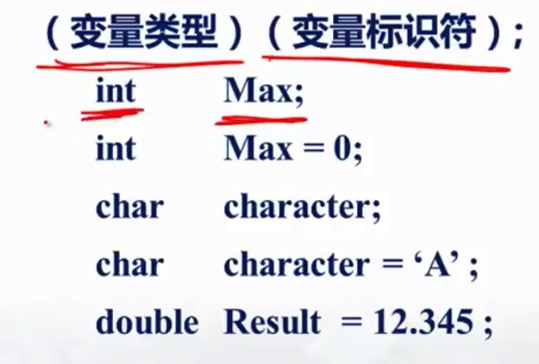
\includegraphics[width=10cm,height=7cm]{variable.jpg}
\caption{变量定义格式}
\hspace{0.05in}
\end{figure}
定义变量起到的作用:在内存中找到一片存储空间,将其命名为变量名,将变量数字存储到存储空间中,并记录存储空间的初始地址。

3. C中的数据类型:
\begin{figure}[!htb]
\centering
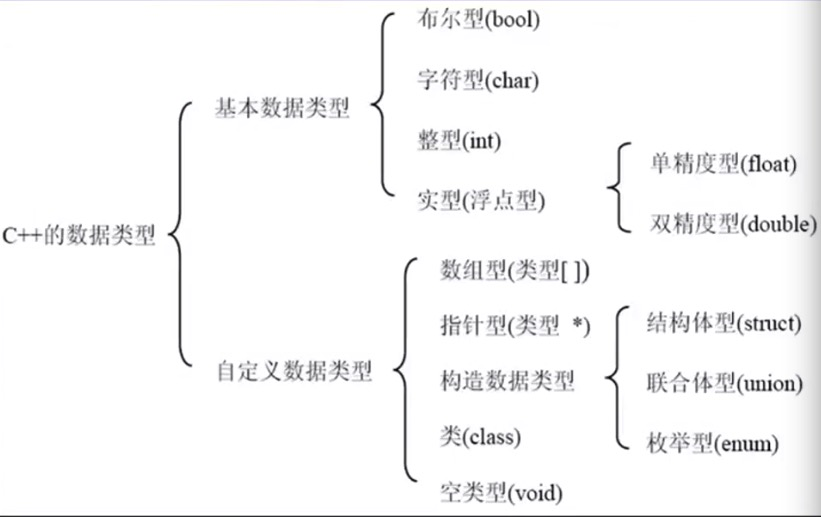
\includegraphics[width=10cm,height=7cm]{datatype.jpg}
\caption{C语言中的数据类型}
\hspace{0.05in}
\end{figure}
\subsection{整数型}




\subsubsection{类别}
\begin{figure}[!htb]
\centering
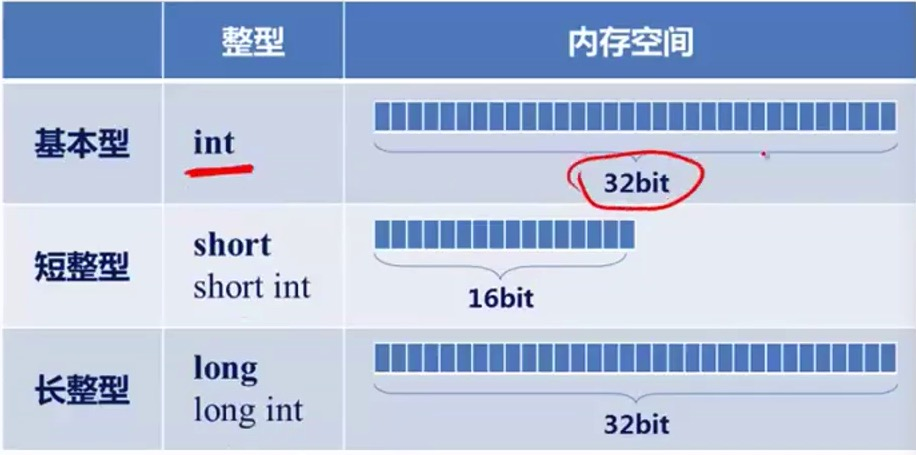
\includegraphics[width=10cm,height=7cm]{inttype.jpg}
\caption{整型数据的分类}
\hspace{0.05in}
\end{figure}

按内存空间的大小区分。(C语言要求long型不短于int型,short型不长于int型,此图表示visual c++中数据的定义,其他编译器int型的字节长度会改变。)
\begin{figure}[!htb]
\centering
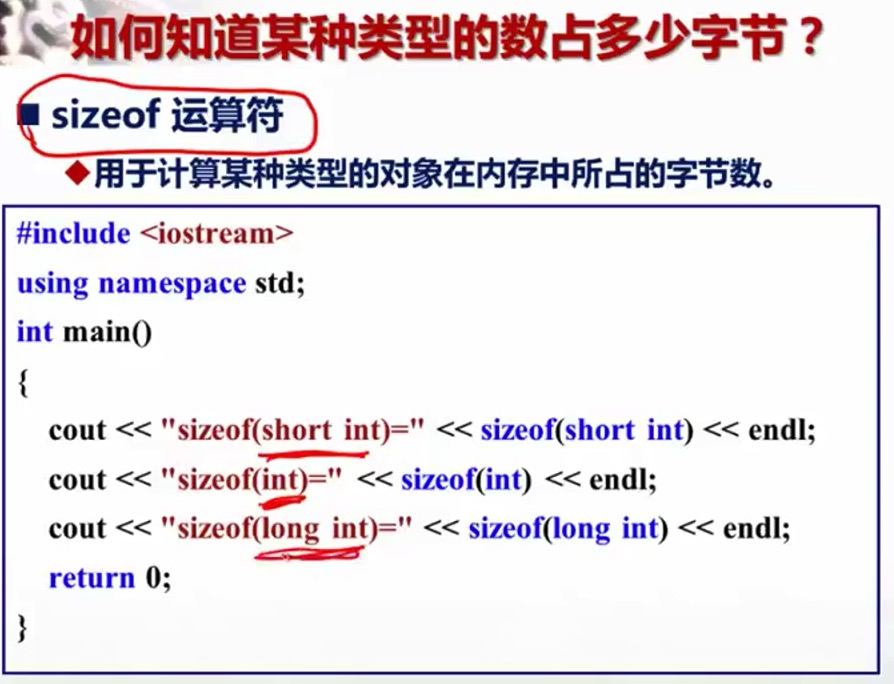
\includegraphics[width=10cm,height=7cm]{printlength.jpg}
\caption{如何知道某种类型数据所占字节数}
\hspace{0.05in}
\end{figure}

Signed可以不写。

\begin{figure}[!htb]
\centering
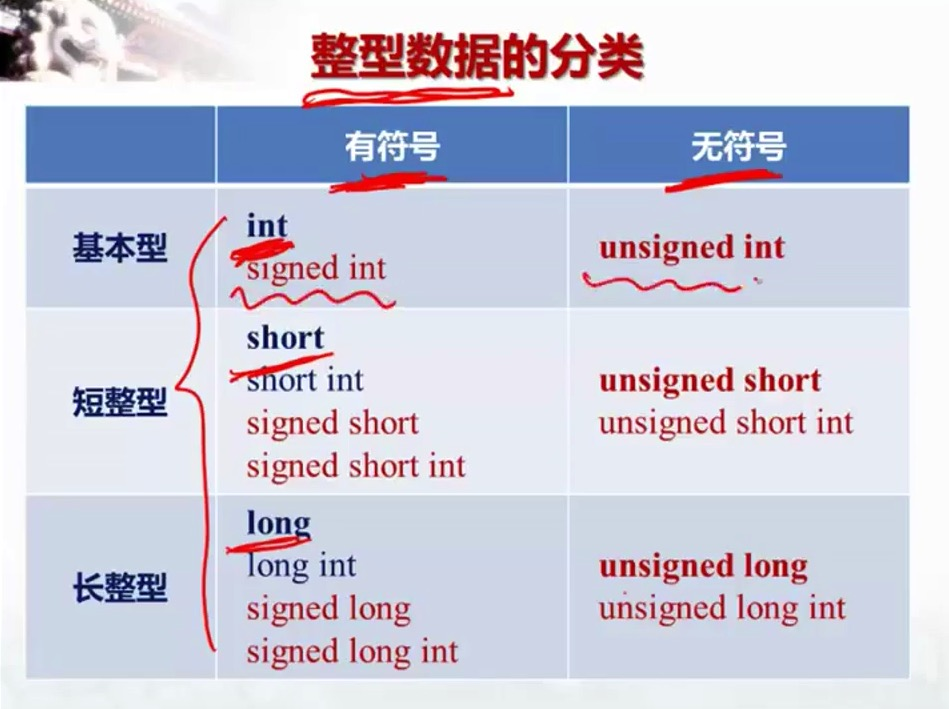
\includegraphics[width=10cm,height=7cm]{inttype1.jpg}
\caption{整型数据的分类}
\hspace{0.05in}
\end{figure}
\subsubsection{存储}
第一位不表示具体数据,只作为符号位,表示数据的正负:1表示负,0表示正。正整数和负整数二进制表示方法不同。计算机中存储的是补码,正整数的补码等于其原码。
\begin{figure}[!htb]
\centering
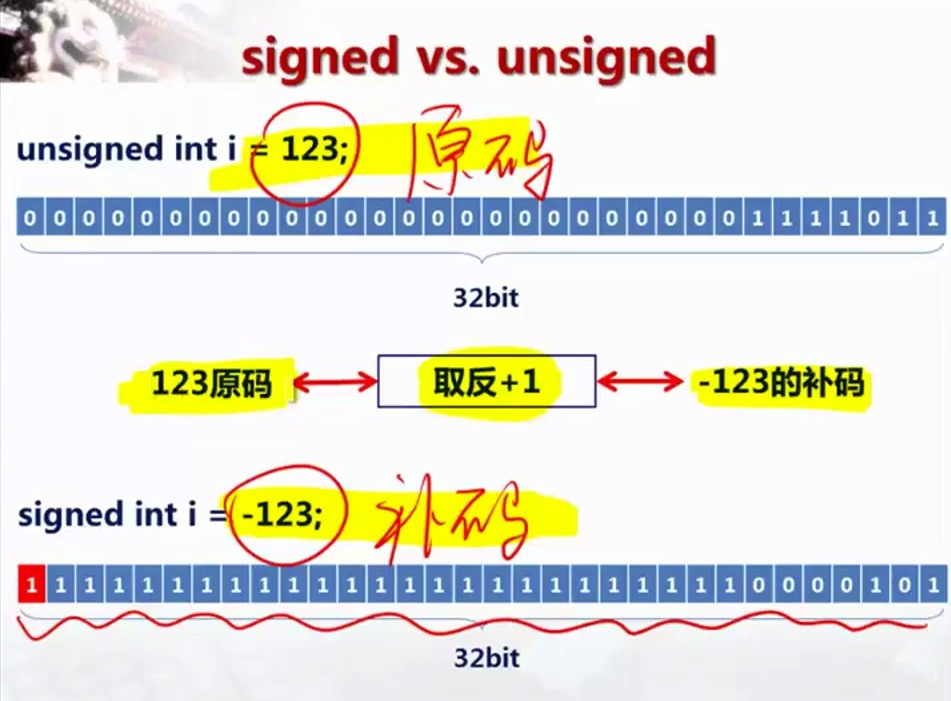
\includegraphics[width=10cm,height=7cm]{buma.jpg}
\caption{如何求补码}
\hspace{0.05in}
\end{figure}
\subsubsection{输入输出}
想知道2进制表示,直接用cout的功能打印出16进制表示就可以。
\begin{figure}[!htb]
\centering
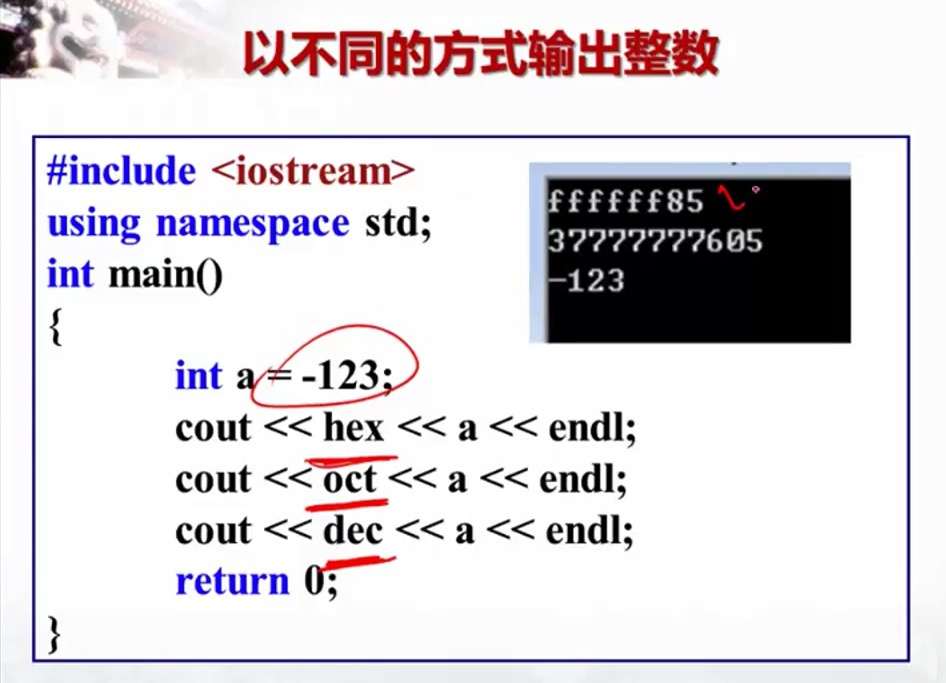
\includegraphics[width=10cm,height=7cm]{16810present.jpg}
\caption{打印一个数的十六,八,十进制表示}
\hspace{0.05in}
\end{figure}

注意:如果不修改,则会一直按该进制输出。
\begin{figure}[!htb]
\centering
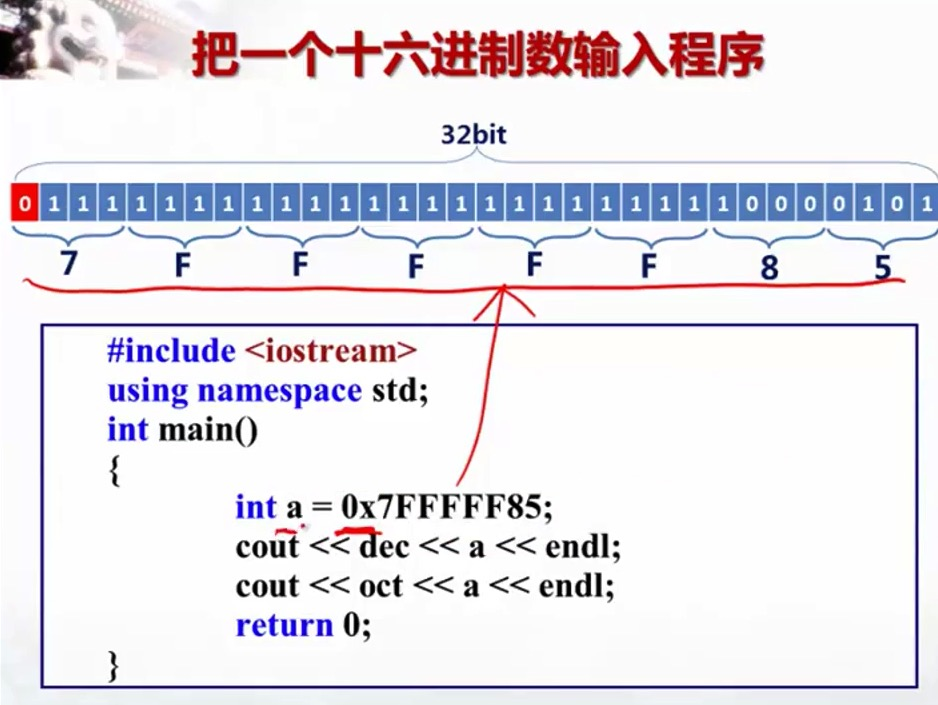
\includegraphics[width=10cm,height=7cm]{16input.jpg}
\caption{输入十六进制数}
\hspace{0.05in}
\end{figure}
0x开头,默认为16进制,0开头的数,默认为8进制,输入二进制数字时,可通过先计算16,8进制再输入。
\subsubsection{最大与最小整数}

\begin{figure}[!htb]
\centering
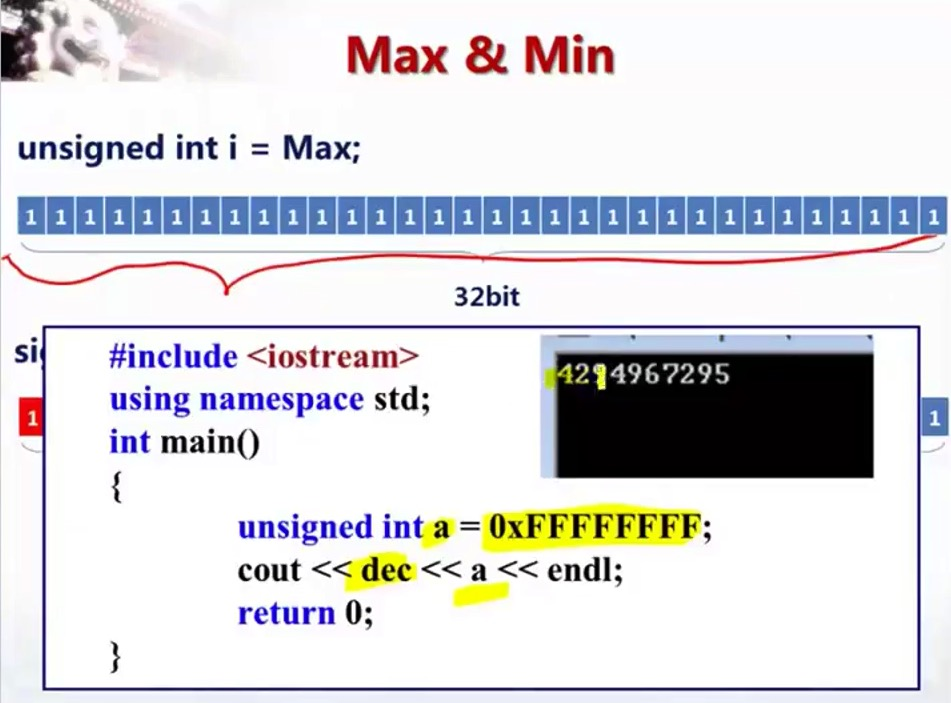
\includegraphics[width=10cm,height=7cm]{max.jpg}
\caption{unsigned int型数据定义的最大值}
\hspace{0.05in}
\end{figure}

有符号数的最大值为:2147483647,最小值为;-2147483648。
\begin{figure}[!htb]
\centering
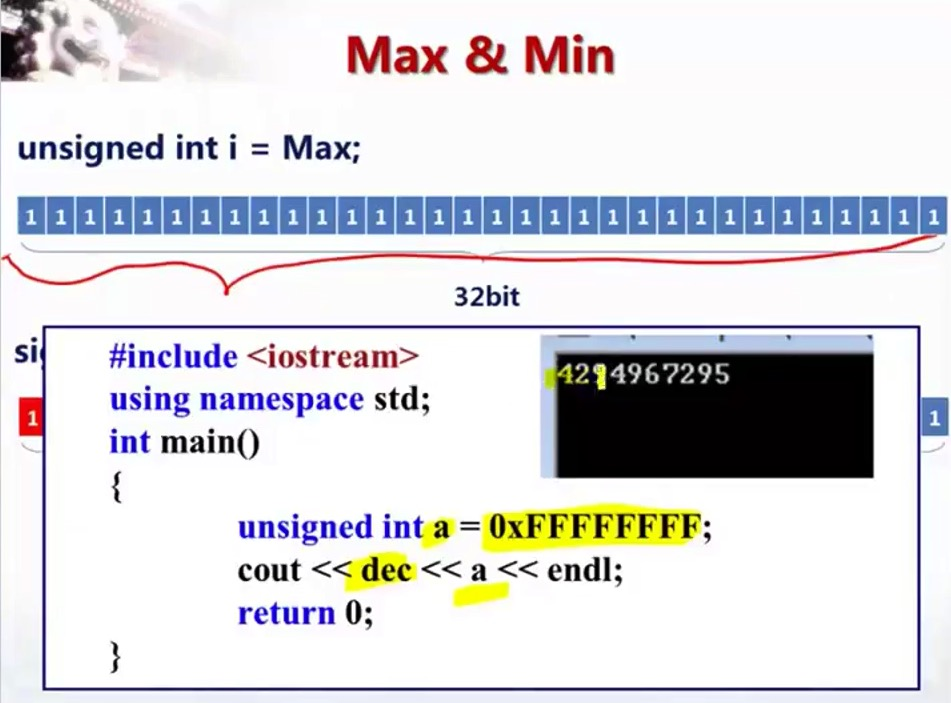
\includegraphics[width=10cm,height=7cm]{max.jpg}
\caption{int型数据定义的最小值}
\hspace{0.05in}
\end{figure}

\begin{figure}[!htb]
\centering
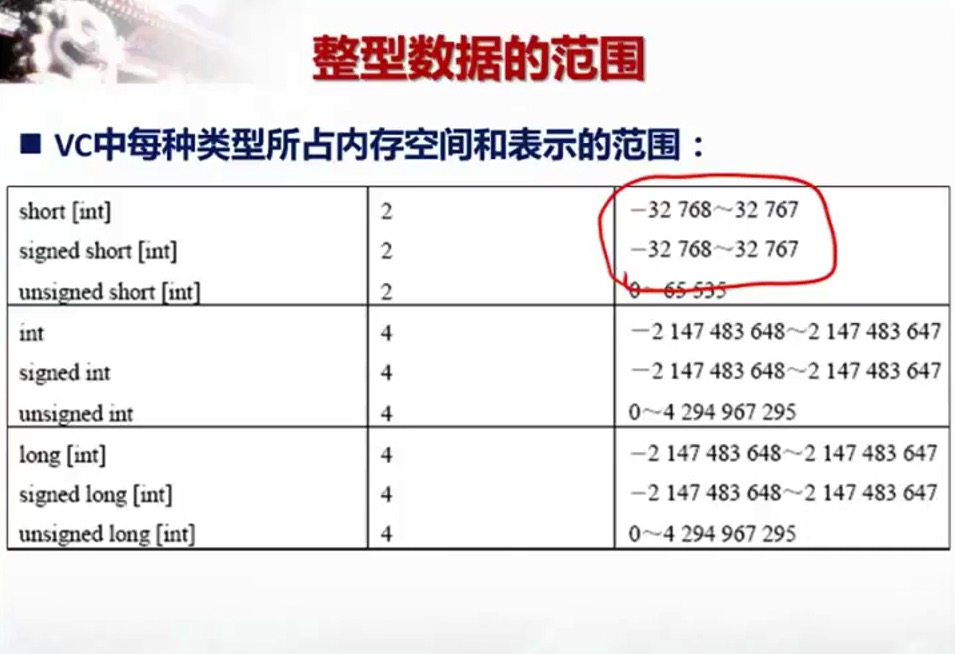
\includegraphics[width=10cm,height=7cm]{maxandmin.jpg}
\caption{各种数据类型的最大值和最小值}
\hspace{0.05in}
\end{figure}

\subsection{浮点型}
浮点型又称为实型
\begin{figure}[!htb]
\centering
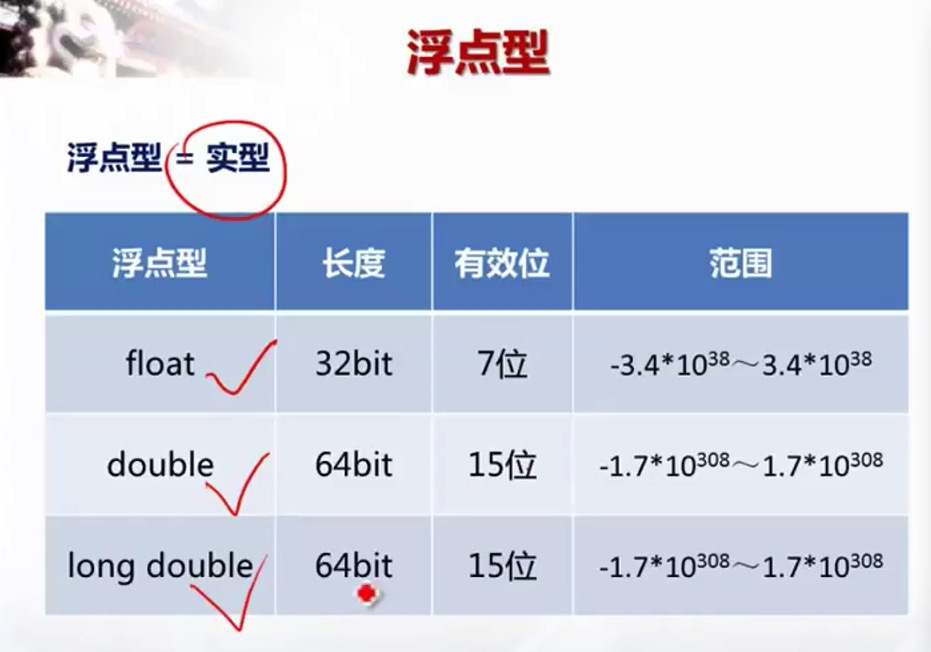
\includegraphics[width=10cm,height=7cm]{fudiantypes.jpg}
\caption{不同类型的浮点型数据}
\hspace{0.05in}
\end{figure}
如果不设置精度,cout默认精度为6位。超出字符类型精度外的位数会输出错误的数据。
\begin{figure}[!htb]
\centering
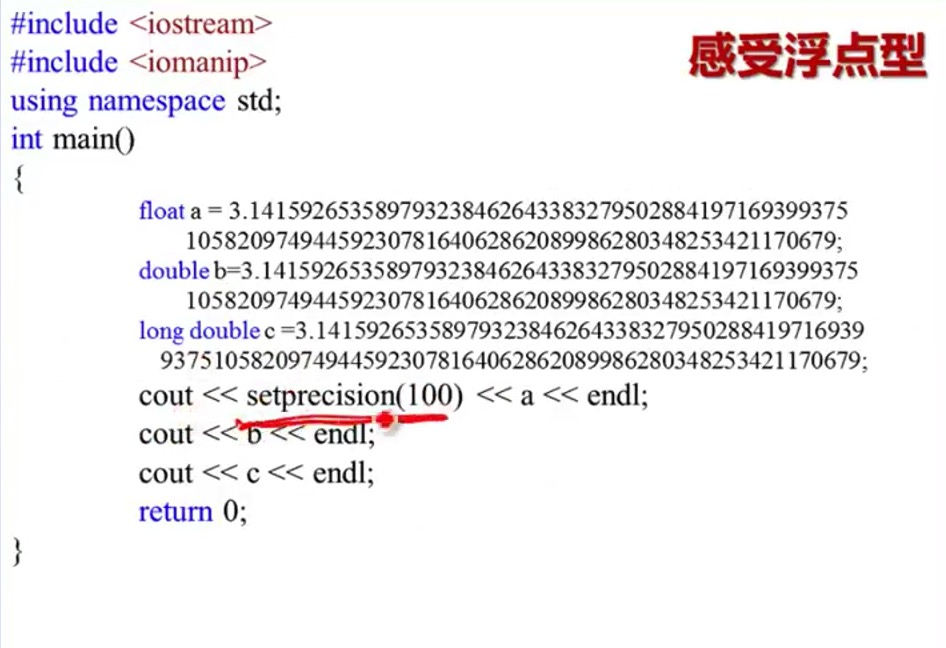
\includegraphics[width=10cm,height=7cm]{coutsetprecision.jpg}
\caption{cout设置输出精度}
\hspace{0.05in}
\end{figure}
float数据在内存中的存储方式如下,其他的类型不再细讲。
\begin{figure}[!htb]
\centering
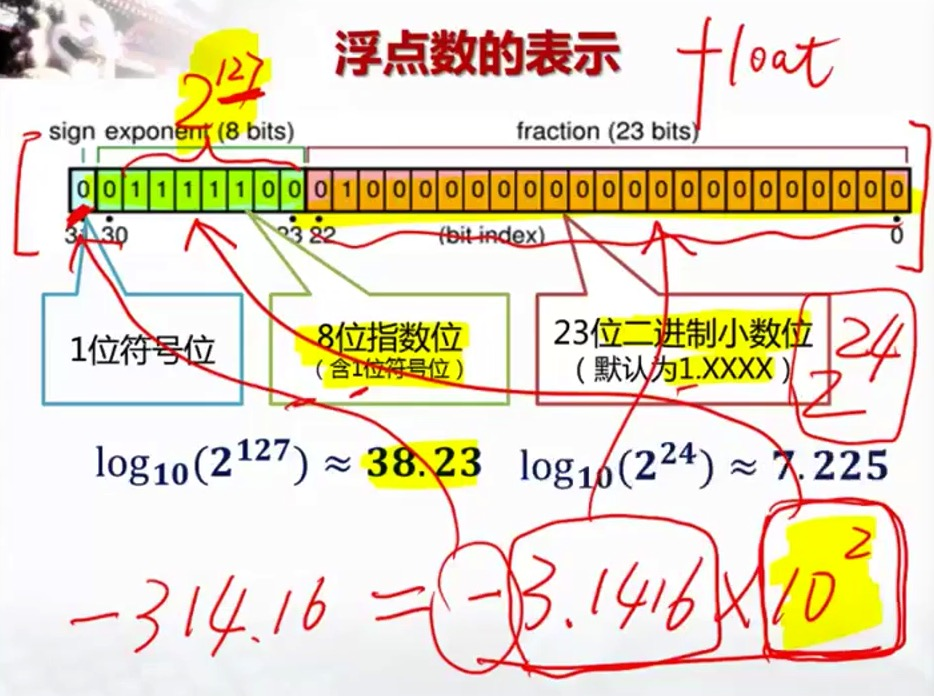
\includegraphics[width=10cm,height=7cm]{floatpresent.jpg}
\caption{float型数据的存储方式}
\hspace{0.05in}
\end{figure}
\subsection{字符型}
一个字符型占一个字节,一个字符在内存中转换成相应的数字来保存。字符型数据可以和整型数据相互赋值,也可以和整数一样进行运算。
\begin{figure}[!htb]
\centering
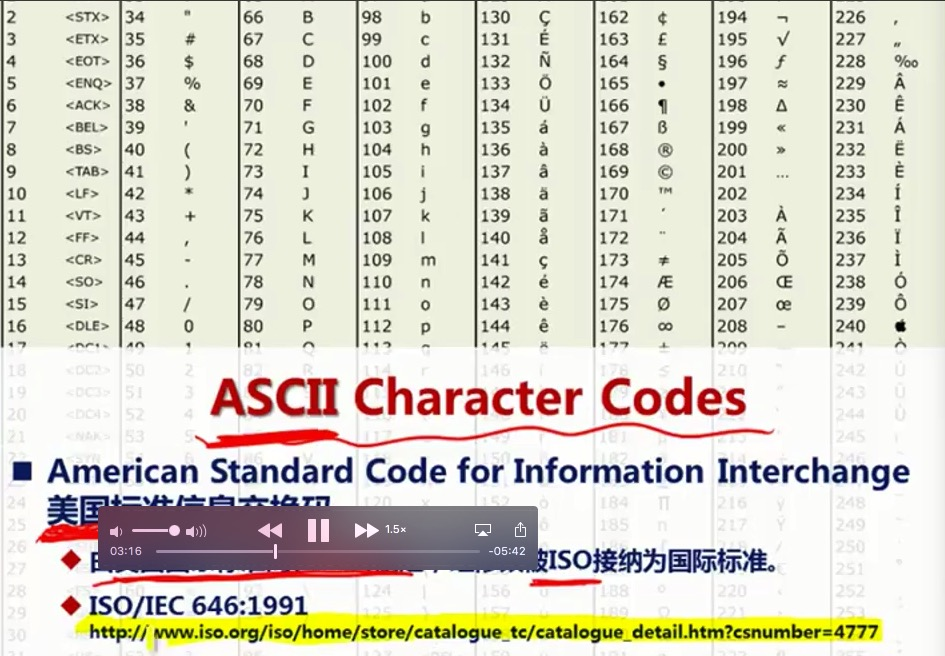
\includegraphics[width=10cm,height=7cm]{ascii.jpg}
\caption{ASCII码}
\hspace{0.05in}
\end{figure}

\begin{figure}[!htb]
\centering
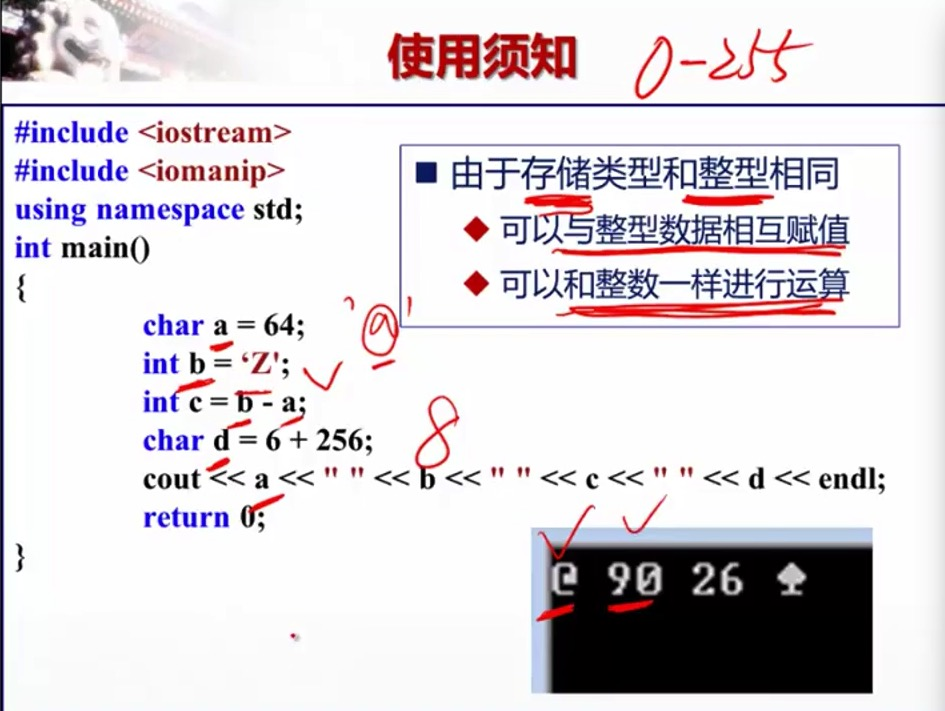
\includegraphics[width=10cm,height=7cm]{intandchar.jpg}
\caption{整型和字符型的运算}
\hspace{0.05in}
\end{figure}
特殊字符:转义字符,转义字符的功能见下图:
\begin{figure}[!htb]
\centering
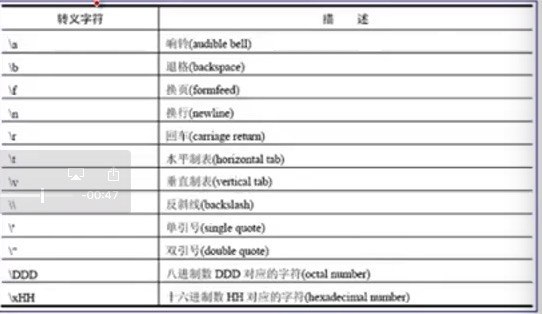
\includegraphics[width=10cm,height=7cm]{zhuanyichar.jpg}
\caption{整型和字符型的运算}
\hspace{0.05in}
\end{figure}

\subsection{布尔型}
用于存``真”和``假”,只占一个字节,其值只能为1或0,1代表true,0代表false。
\begin{figure}[!htb]
\centering
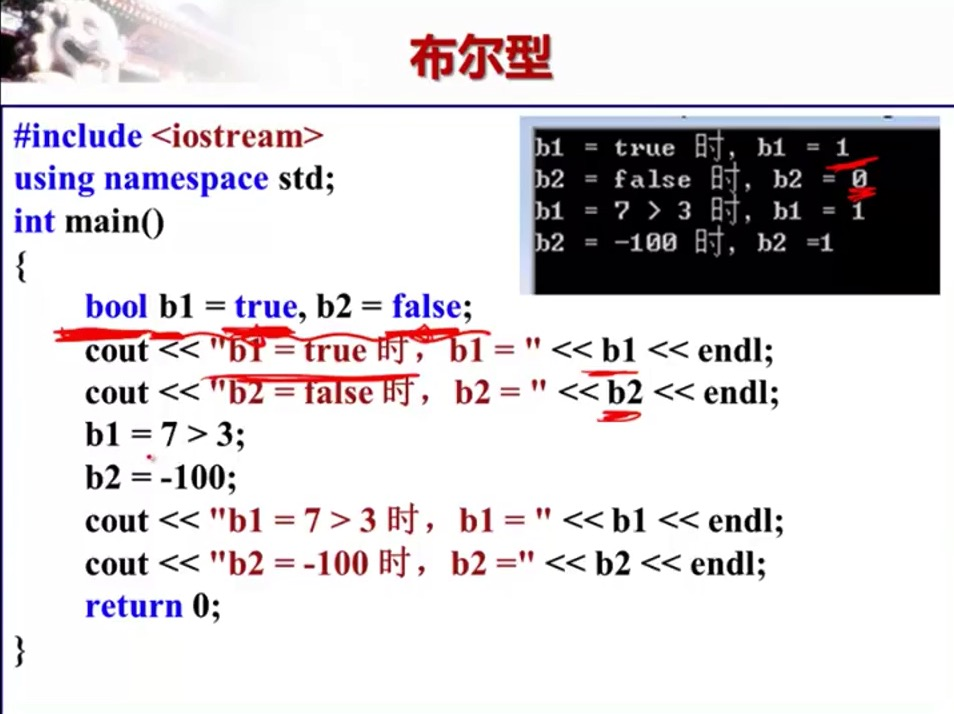
\includegraphics[width=10cm,height=7cm]{bool.jpg}
\caption{布尔型``非0即1”}
\hspace{0.05in}
\end{figure}

\subsection{常数}
常量:程序运行中,其值不变的量,有字面常量和符号常量两种(定义方法如下图)。也是有数据类型的。
\begin{figure}[!htb]
\centering
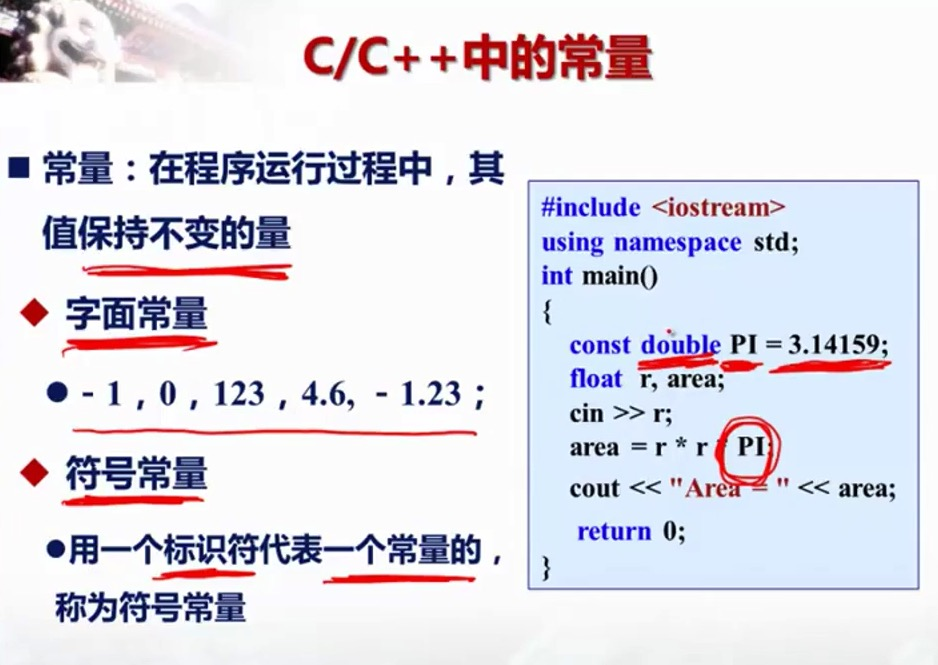
\includegraphics[width=10cm,height=7cm]{definechangliang.jpg}
\caption{符号常量PI的定义方法}
\hspace{0.05in}
\end{figure}

常量的类型靠后缀来区分:

\begin{figure}[!htb]
\centering
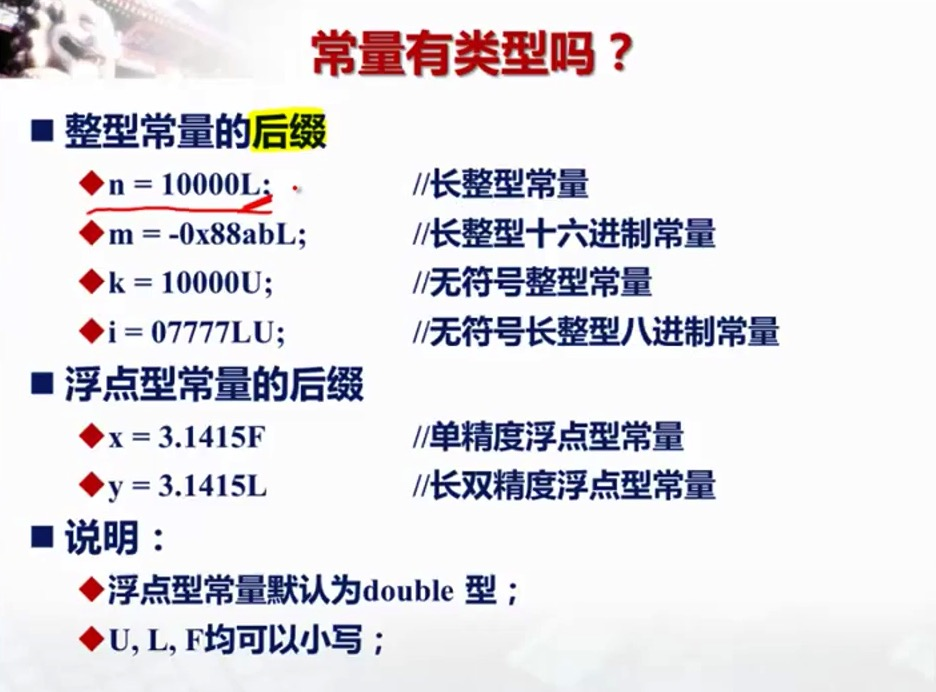
\includegraphics[width=10cm,height=7cm]{changliangtype.jpg}
\caption{符号常量PI的定义方法}
\hspace{0.05in}
\end{figure}
\subsection{变量命名}

\begin{figure}[!htb]
\centering
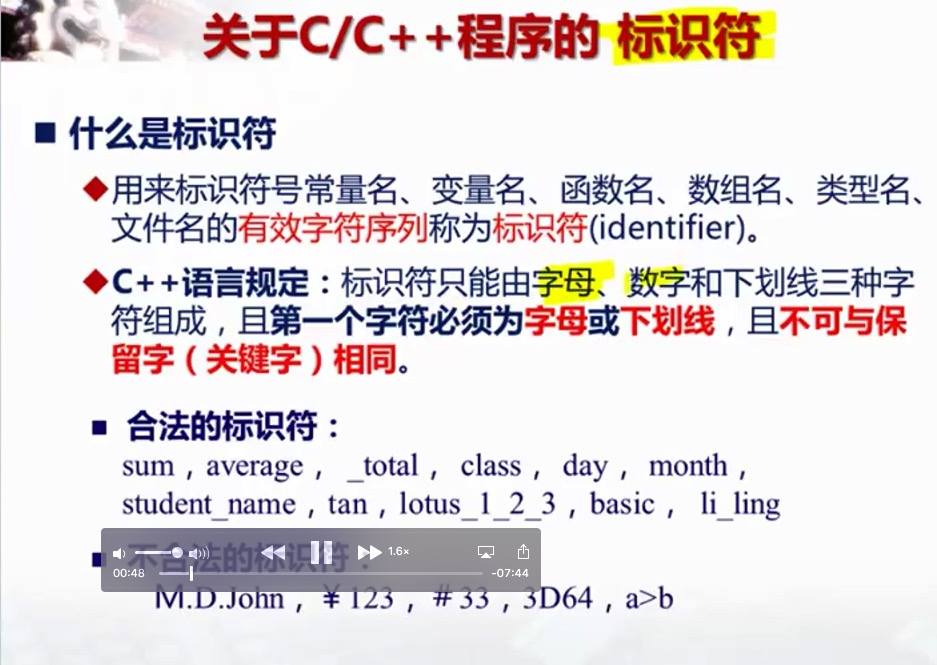
\includegraphics[width=10cm,height=7cm]{bianliangname.jpg}
\caption{变量标识符的定义}
\hspace{0.05in}
\end{figure}
现在常用的两种命名法:匈牙利命名法和驼峰命名法:
\begin{figure}[!htb]
\centering

\includegraphics[width=10cm,height=7cm]{xiongyali.jpg}
\caption{匈牙利命名法}
\hspace{0.05in}
\end{figure}
\begin{figure}[!htb]
\centering

\includegraphics[width=10cm,height=7cm]{tuofeng.jpg}
\caption{驼峰命名法}
\hspace{0.05in}
\end{figure}


\section{c语言中的运算成分}
\subsection{赋值运算}
\subsection{算术运算}
\subsection{自增自减运算}
\subsection{关系运算}
\subsection{逻辑运算和混合运算}
\subsection{逗号,条件,强转}
\subsection{位运算}



\end{document}
